\chapter{Технологическая часть}

В этой части будут выбраны средства реализации разрабатываемого ПО, проведено модульное и функциональное тестирование.

\section{Средства реализации}

В качестве основного языка программирования для реализации ПО был выбран Go~\cite{go}. Этот язык был выбран так как:

\begin{itemize}
	\item средствами языка можно реализовать все спроектированные алгоритмы;
	\item в стандартной библиотеке языка есть средства для реализации всех спроектированных структур.
\end{itemize}

Для графического интерфейса была выбрана библиотека Fyne~\cite{fyne}, так как:

\begin{itemize}
	\item средств библиотеки достаточно для работы с растровой графикой и вывода её на экран;
	\item библиотека является кроссплатформенной.
\end{itemize}

\section{Модульное тестирование}

Модульное тестирование проводилось с помощью стандартного пакета Go -- testing. 

В качестве меры качества покрытия кода использовалась метрика стандартной утилиты cover входящей в состав Go, которая измеряет покрытие кода как процент от выполненных хотя бы единожды выражений~\cite{cover}.

Тестами были покрыты математические модули, модули матричных преобразований, отсечения и чтения объектов.

Покрытие кода составило \textbf{24.7\%}.

Все модульные тесты были пройдены.

\section{Функциональное тестирование}

В качестве функционального тестирования рассмотрены отдельные изображения, полученные разработанным ПО.

На рисунке~\ref{fig:racurs2} представлены изображения сцены, состоящей из различных объектов с разных ракурсов. В каждом положении направление взгляда было направлен в центр координат.

\begin{figure}[H]
	\centering
	\subfigure[X=-8.03, Y=8.55, Z=-22.07]{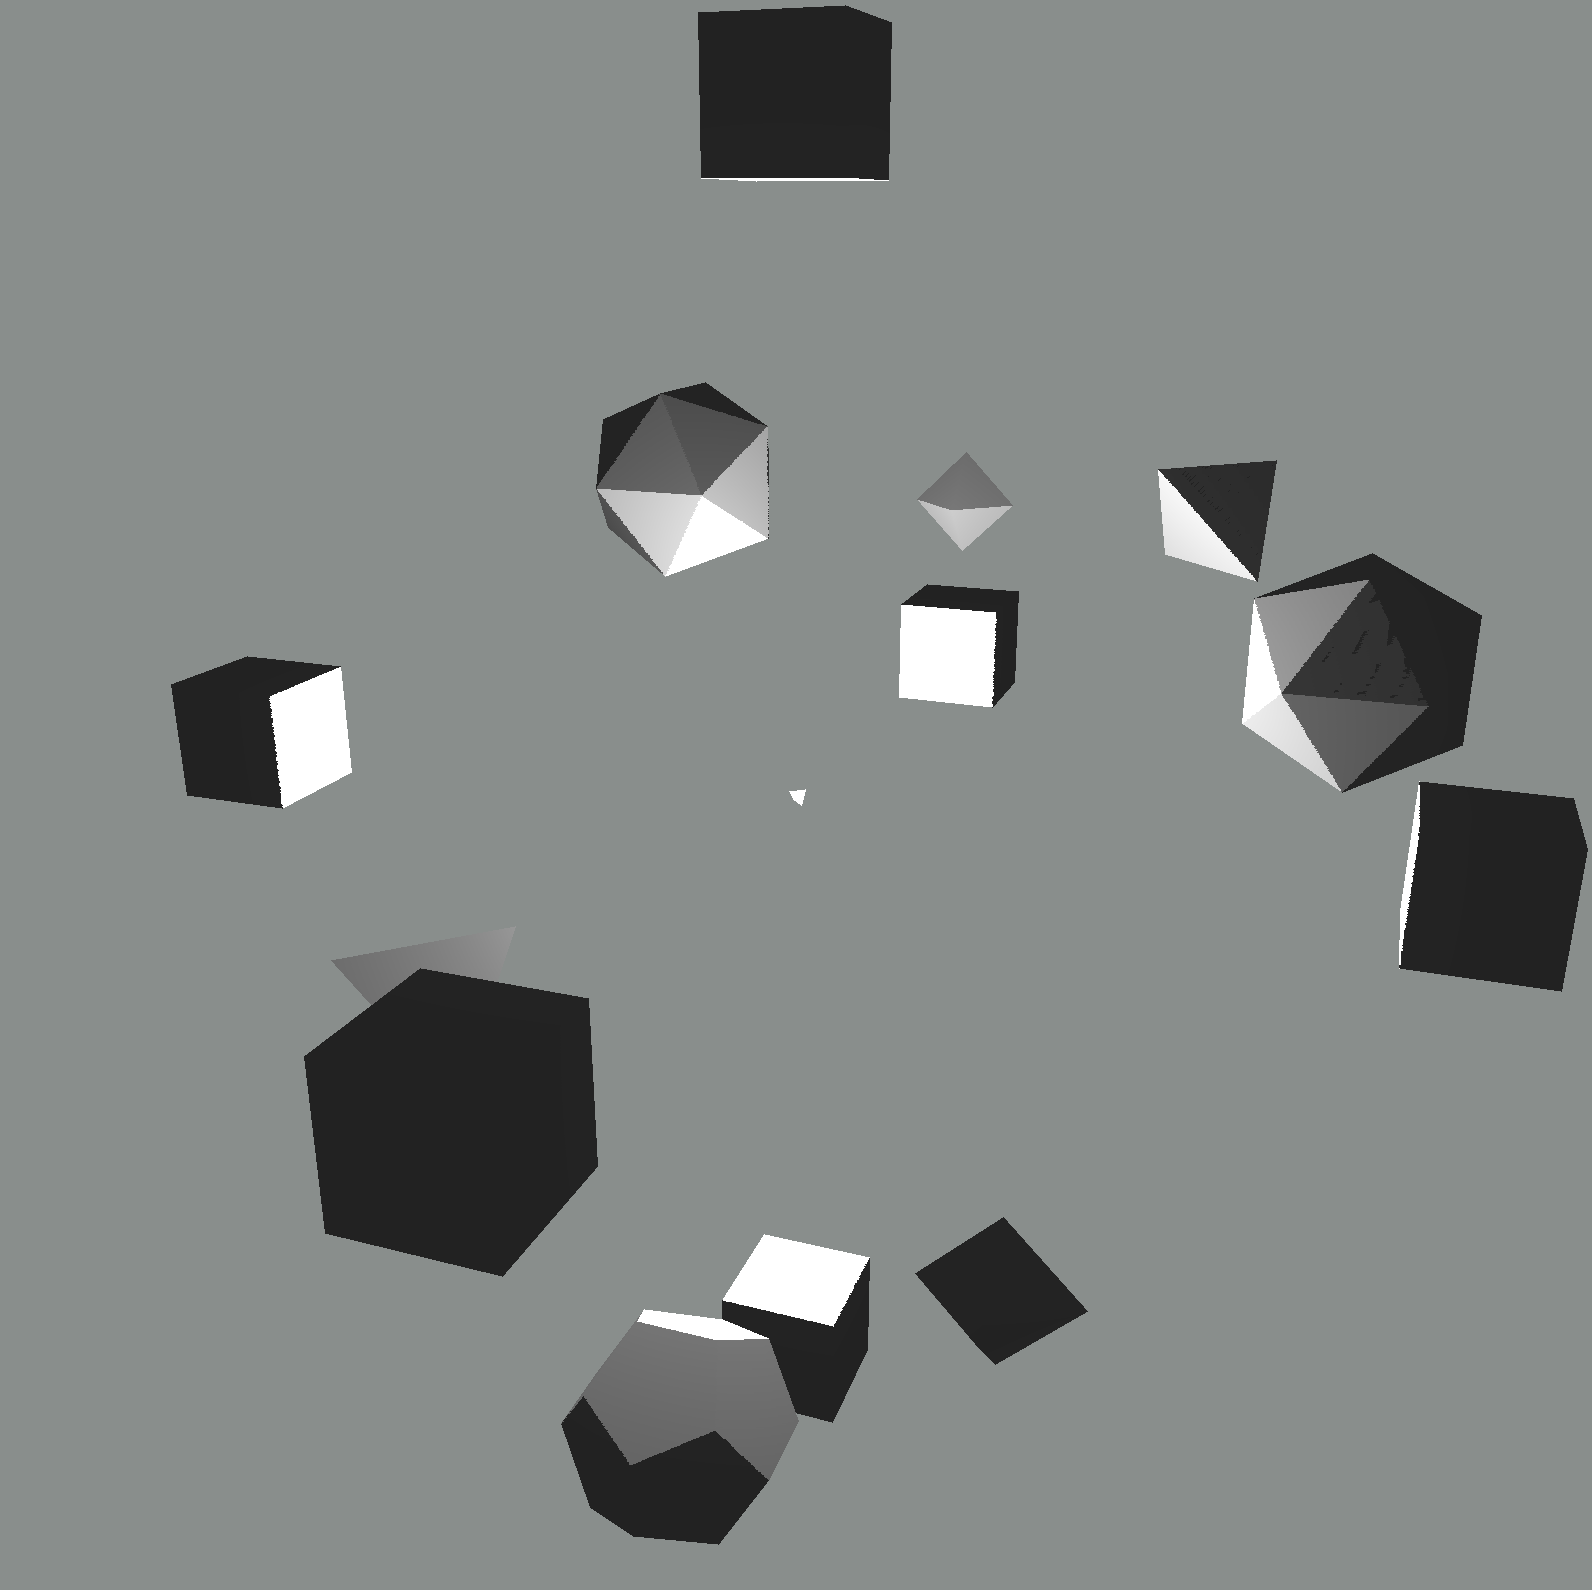
\includegraphics[width=0.3\textwidth]{rakurs1}}
	\hfil
	\subfigure[X=-20.34, Y=12.49, Z=-7.40]{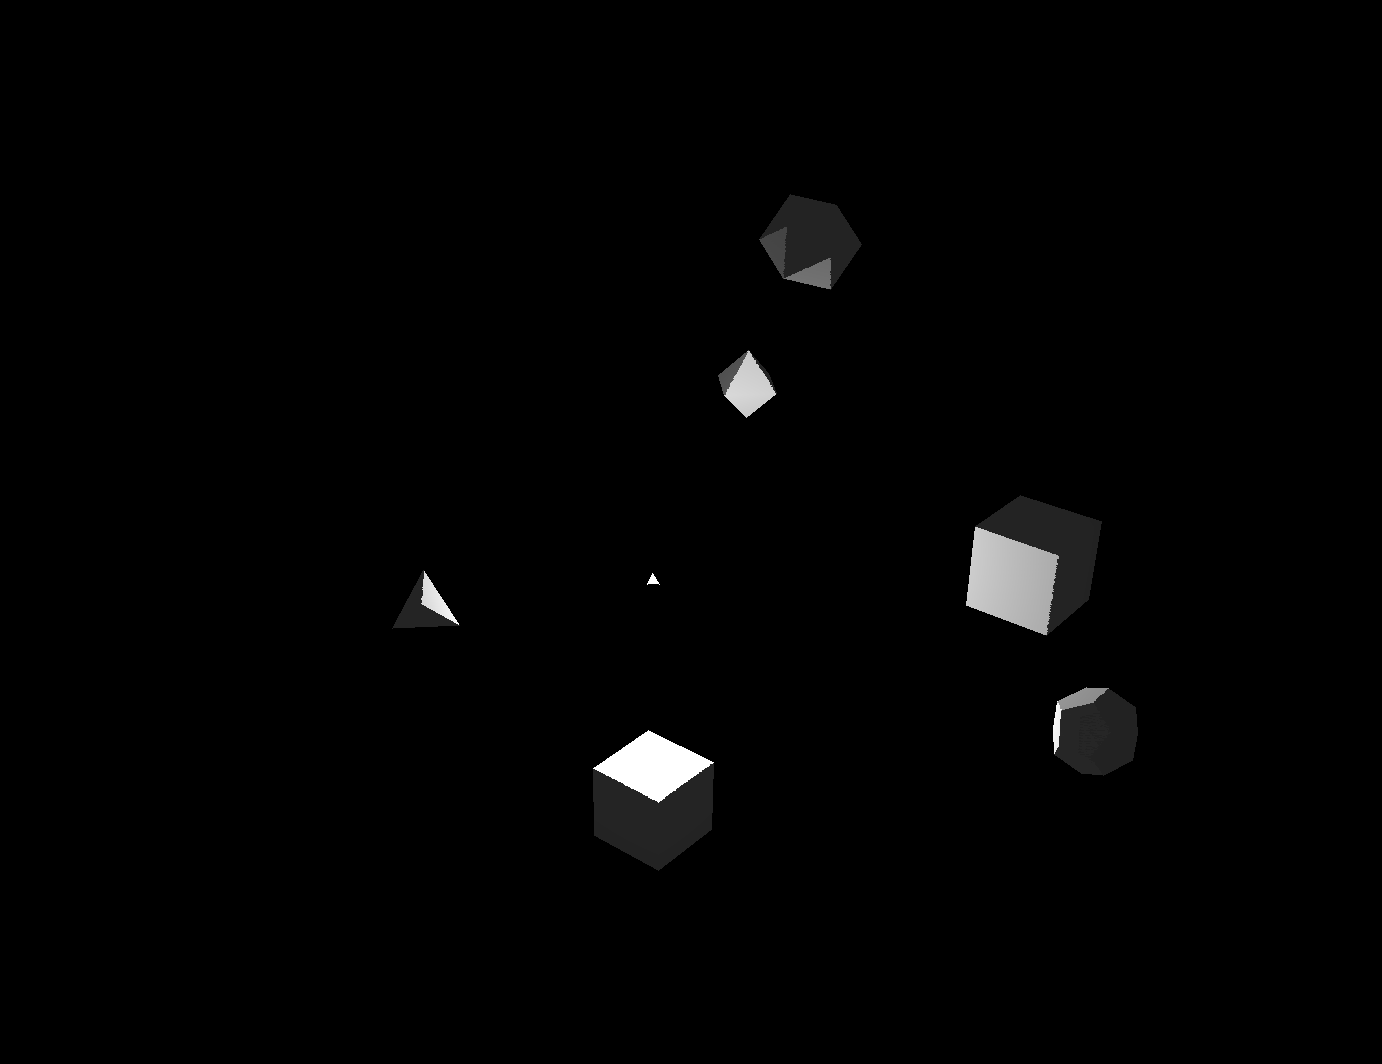
\includegraphics[width=0.3\textwidth]{rakurs2}}
	\hfil
	\subfigure[X=-10.82, Y=12.49, Z=18.75]{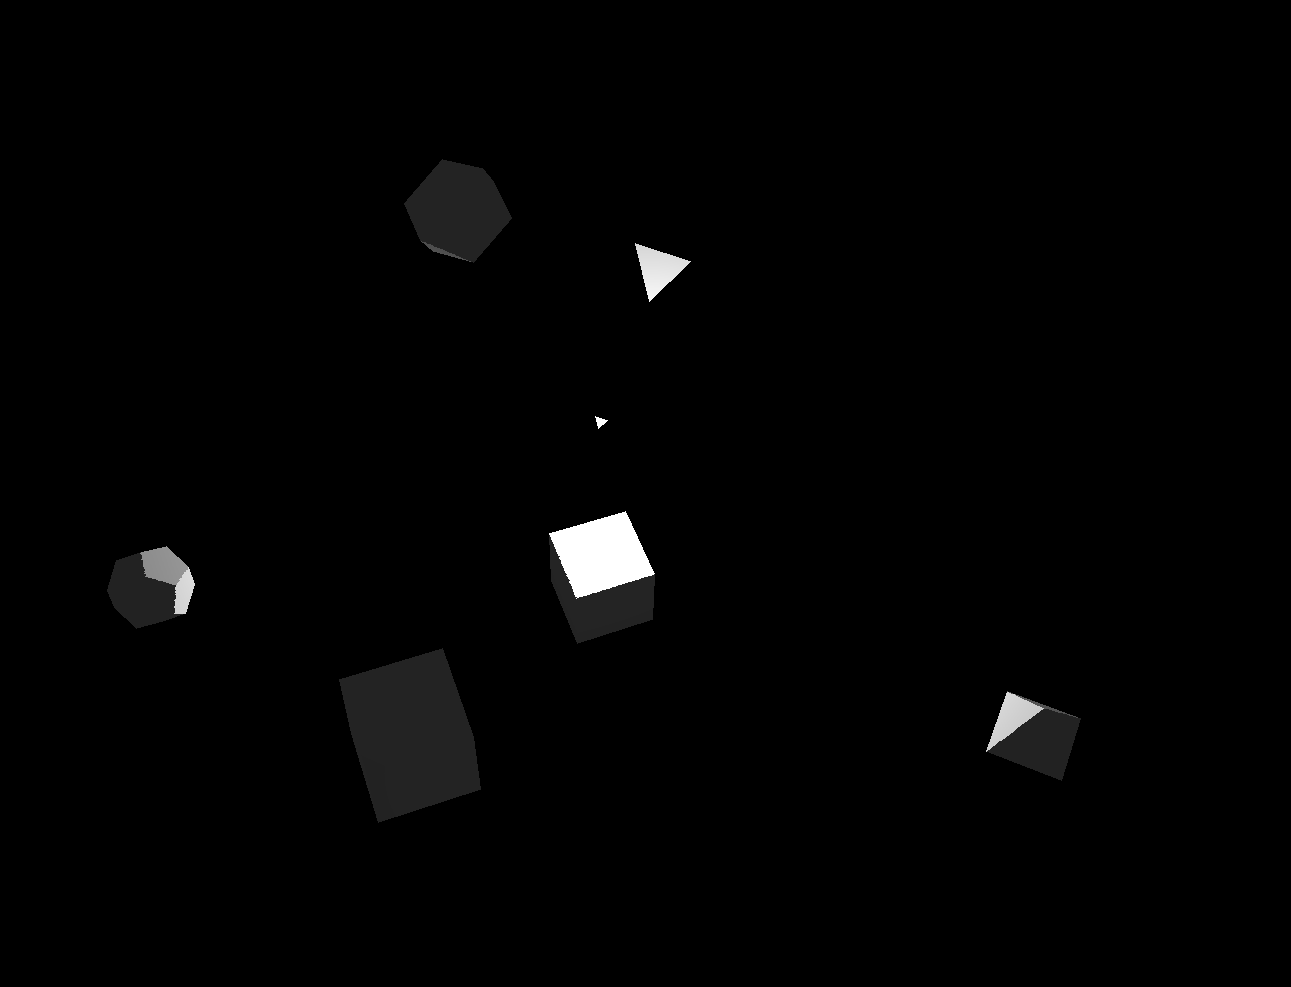
\includegraphics[width=0.3\textwidth]{rakurs3}}
	\caption{<<Сцена с разных ракурсов>>}
	\label{fig:racurs2}
\end{figure}

На рисунке~\ref{fig:shadow128} представлена сцена, на которой демонстрируются тени созданные алгоритмом теневых карт при разрешении буферов 128 на 128, На рисунке~\ref{fig:shadow256} представлена  та же сцена, но при увеличенном разрешении -- 256  на 256, а на рисунке~\ref{fig:shadow512} -- 512 на 512.
Как и ожидалось из-за ограничения в разрешении теневого буфера создаваемые им тени выглядят ступенчато при низком разрешении. При этом чем выше разрешение, тем более гладко выглядят тени

\begin{figure}[H]
	\centering
	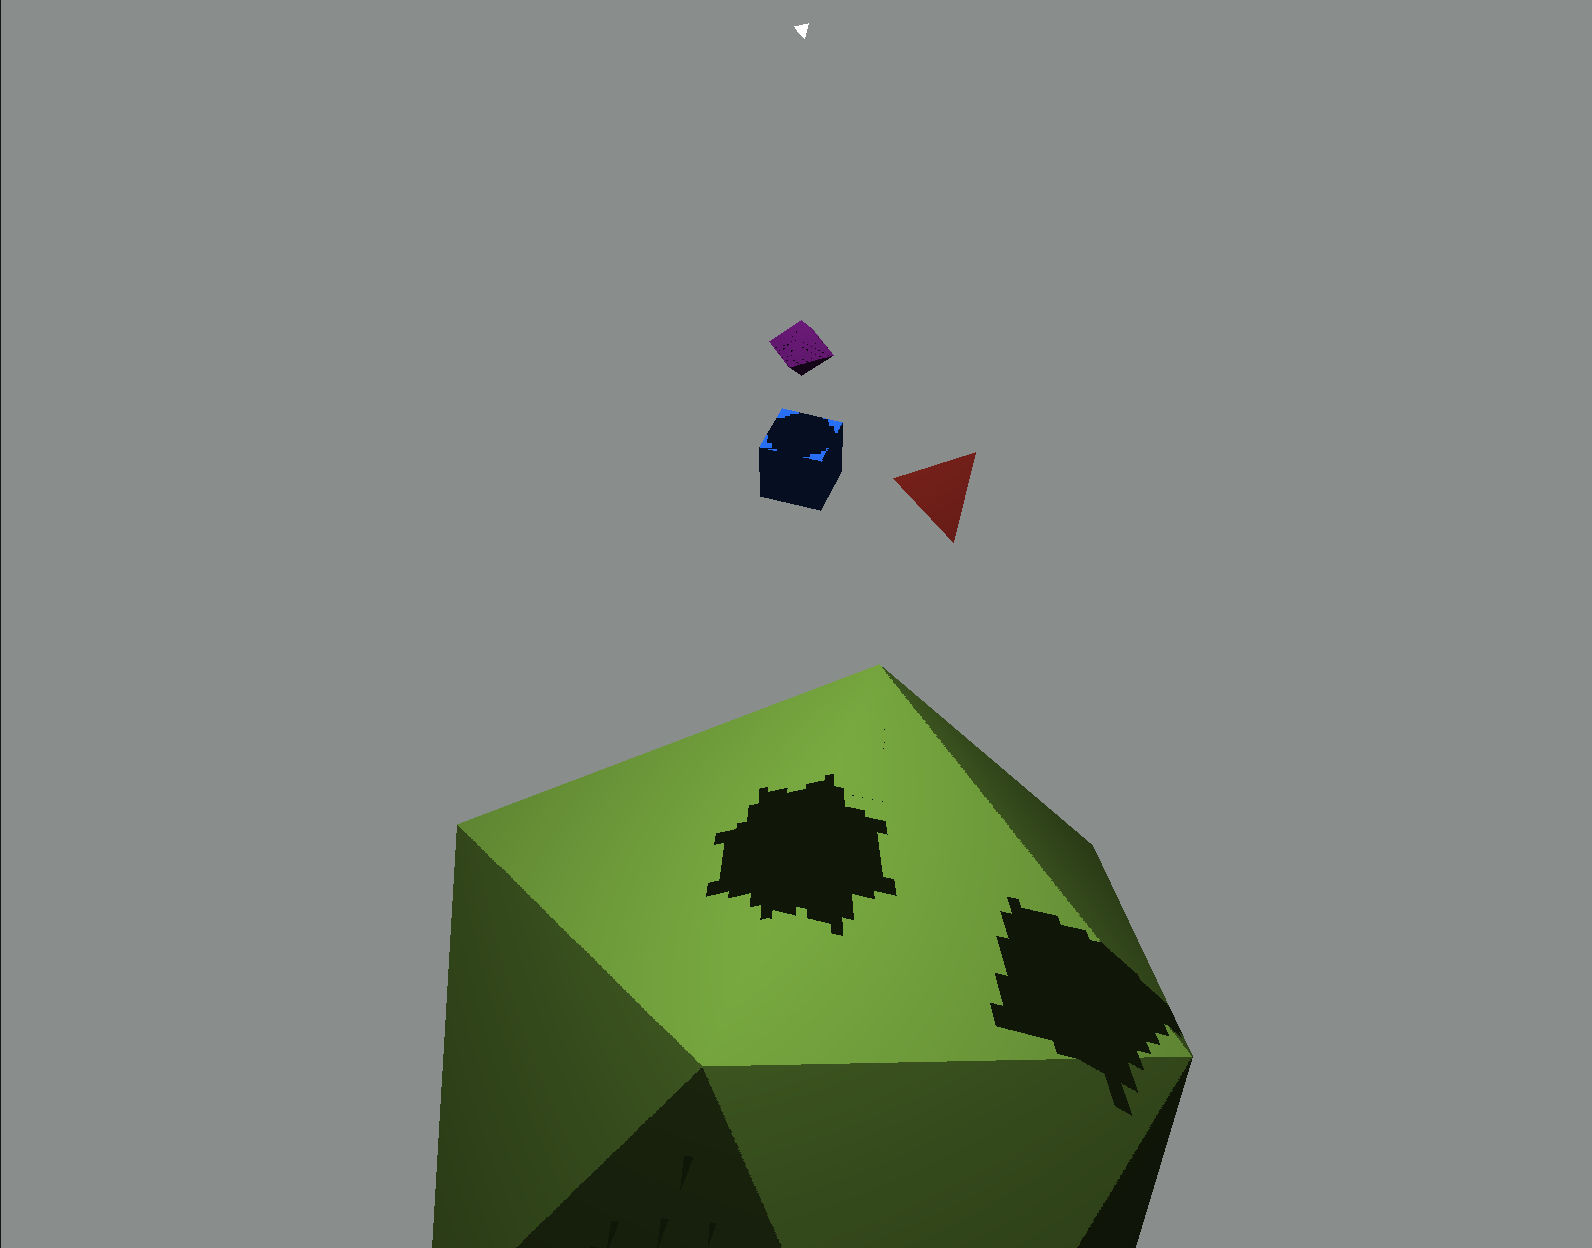
\includegraphics[width=0.6\textwidth]{shadow128}
	\caption{<<Тени созданные теневыми картами при разрешении 128x128>>}
	\label{fig:shadow128}
\end{figure}

\begin{figure}[H]
	\centering
	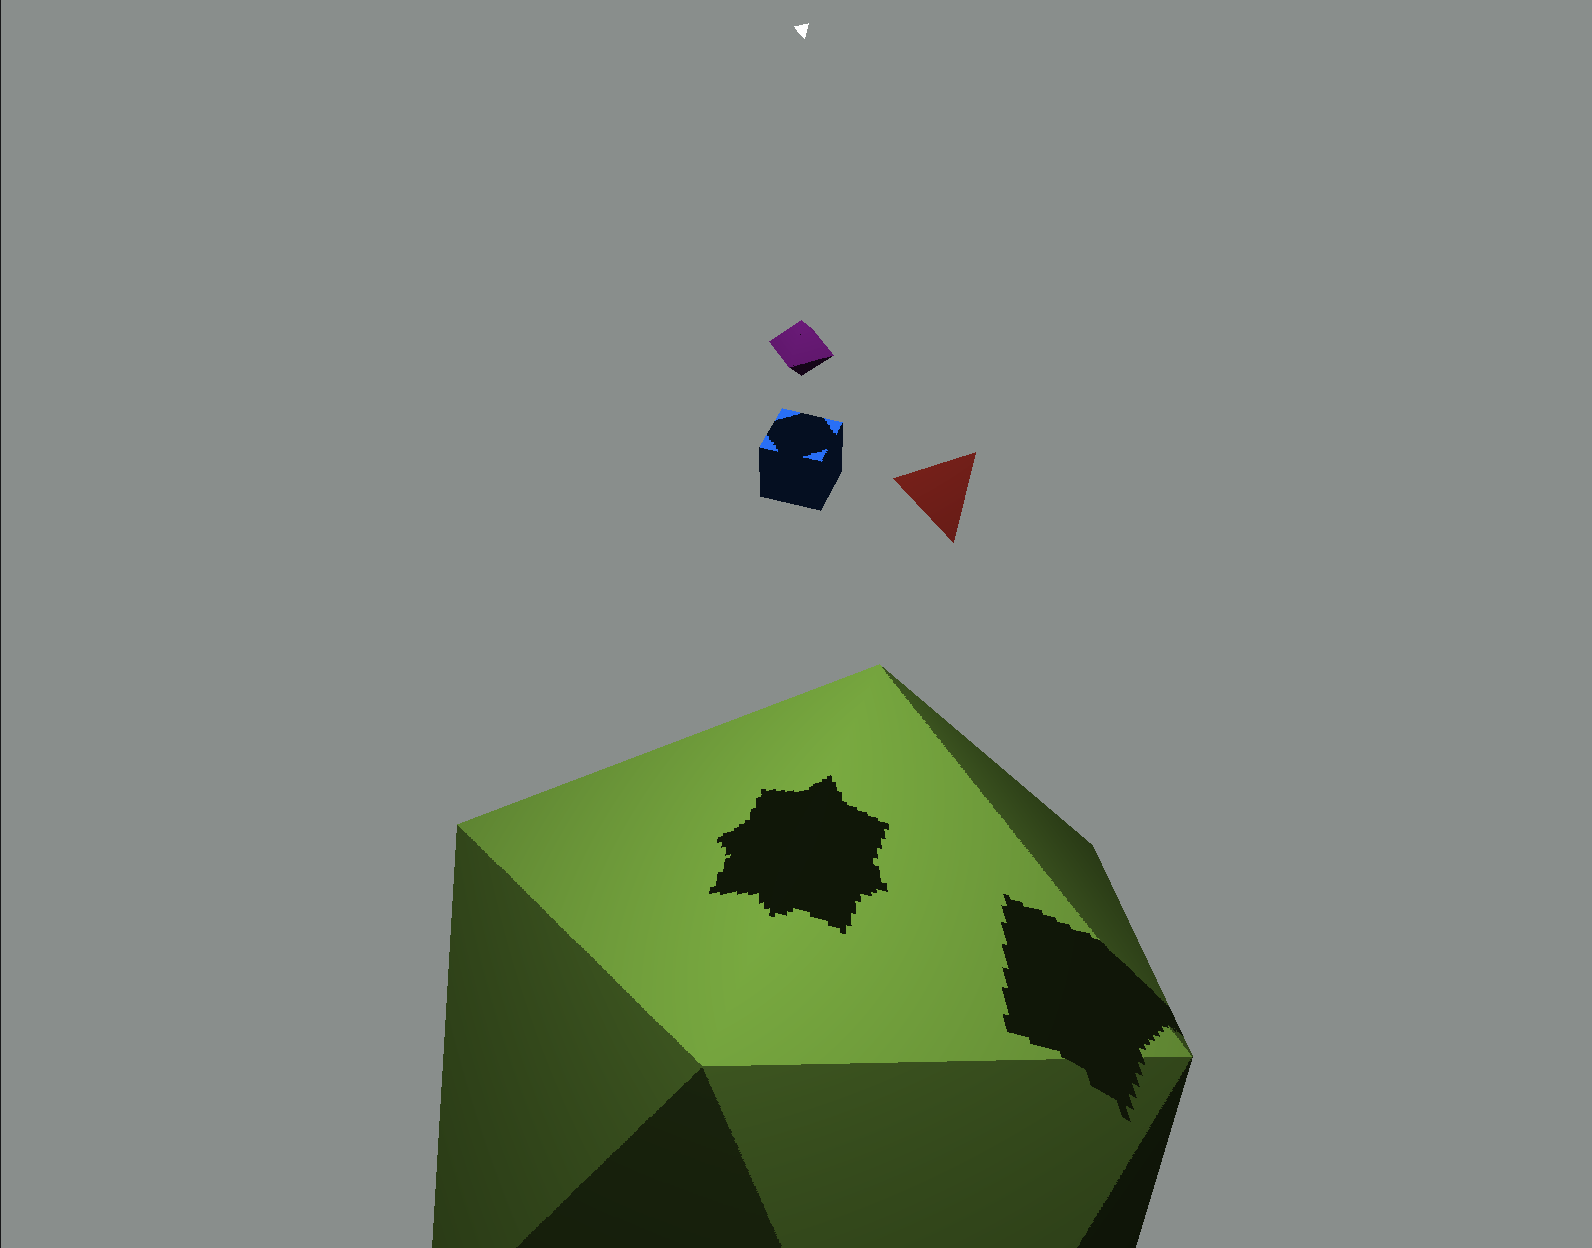
\includegraphics[width=0.6\textwidth]{shadow256}
	\caption{<<Тени созданные теневыми картами при разрешении 256x256>>}
	\label{fig:shadow256}
\end{figure}


\begin{figure}[H]
	\centering
	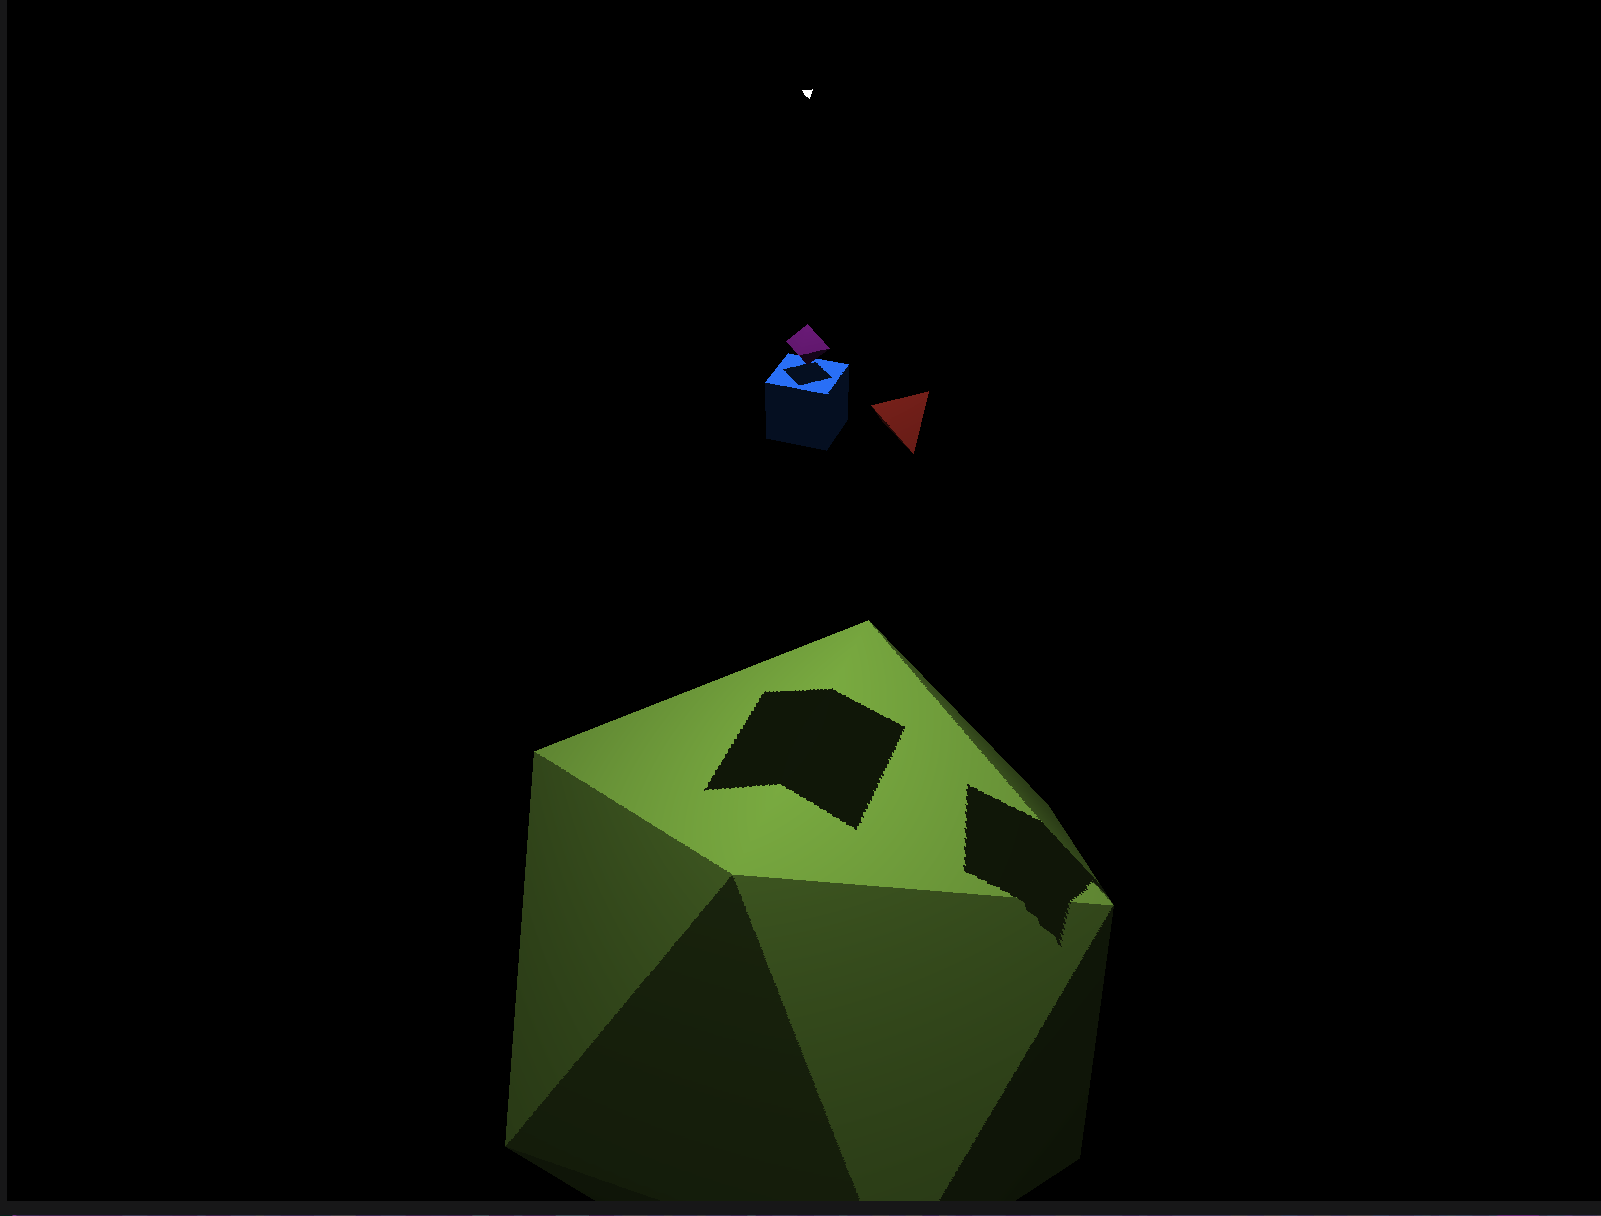
\includegraphics[width=0.6\textwidth]{shadow512}
	\caption{<<Тени созданные теневыми картами при разрешении 512x512>>}
	\label{fig:shadow512}
\end{figure}

На рисунке \ref{fig:light} представлена сцена, которая демонстрирует изменения в освещение объектов и отбрасываемых ими тенях при изменении положения точечного источника.

\begin{figure}[H]
	\centering
	\subfigure[X=0, Y10, Z=0]{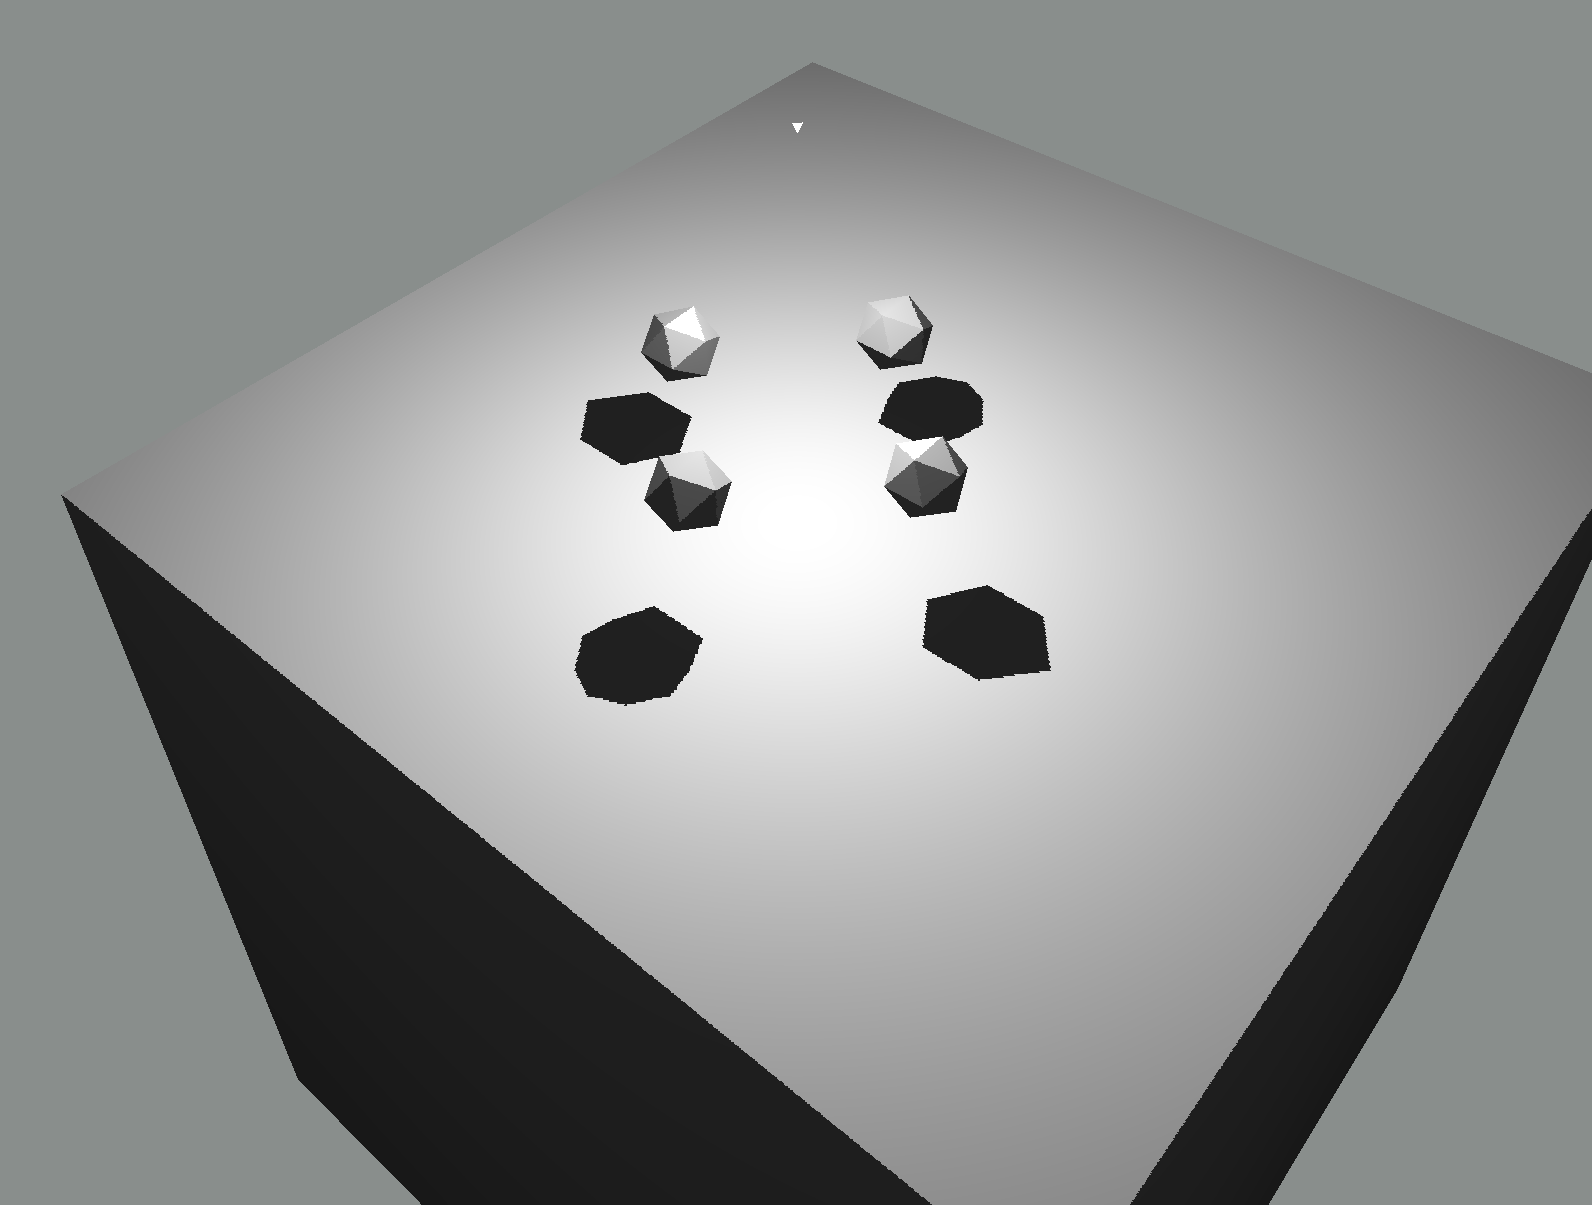
\includegraphics[width=0.3\textwidth]{light1}}
	\hfil
	\subfigure[X=10, Y=10, Z=0]{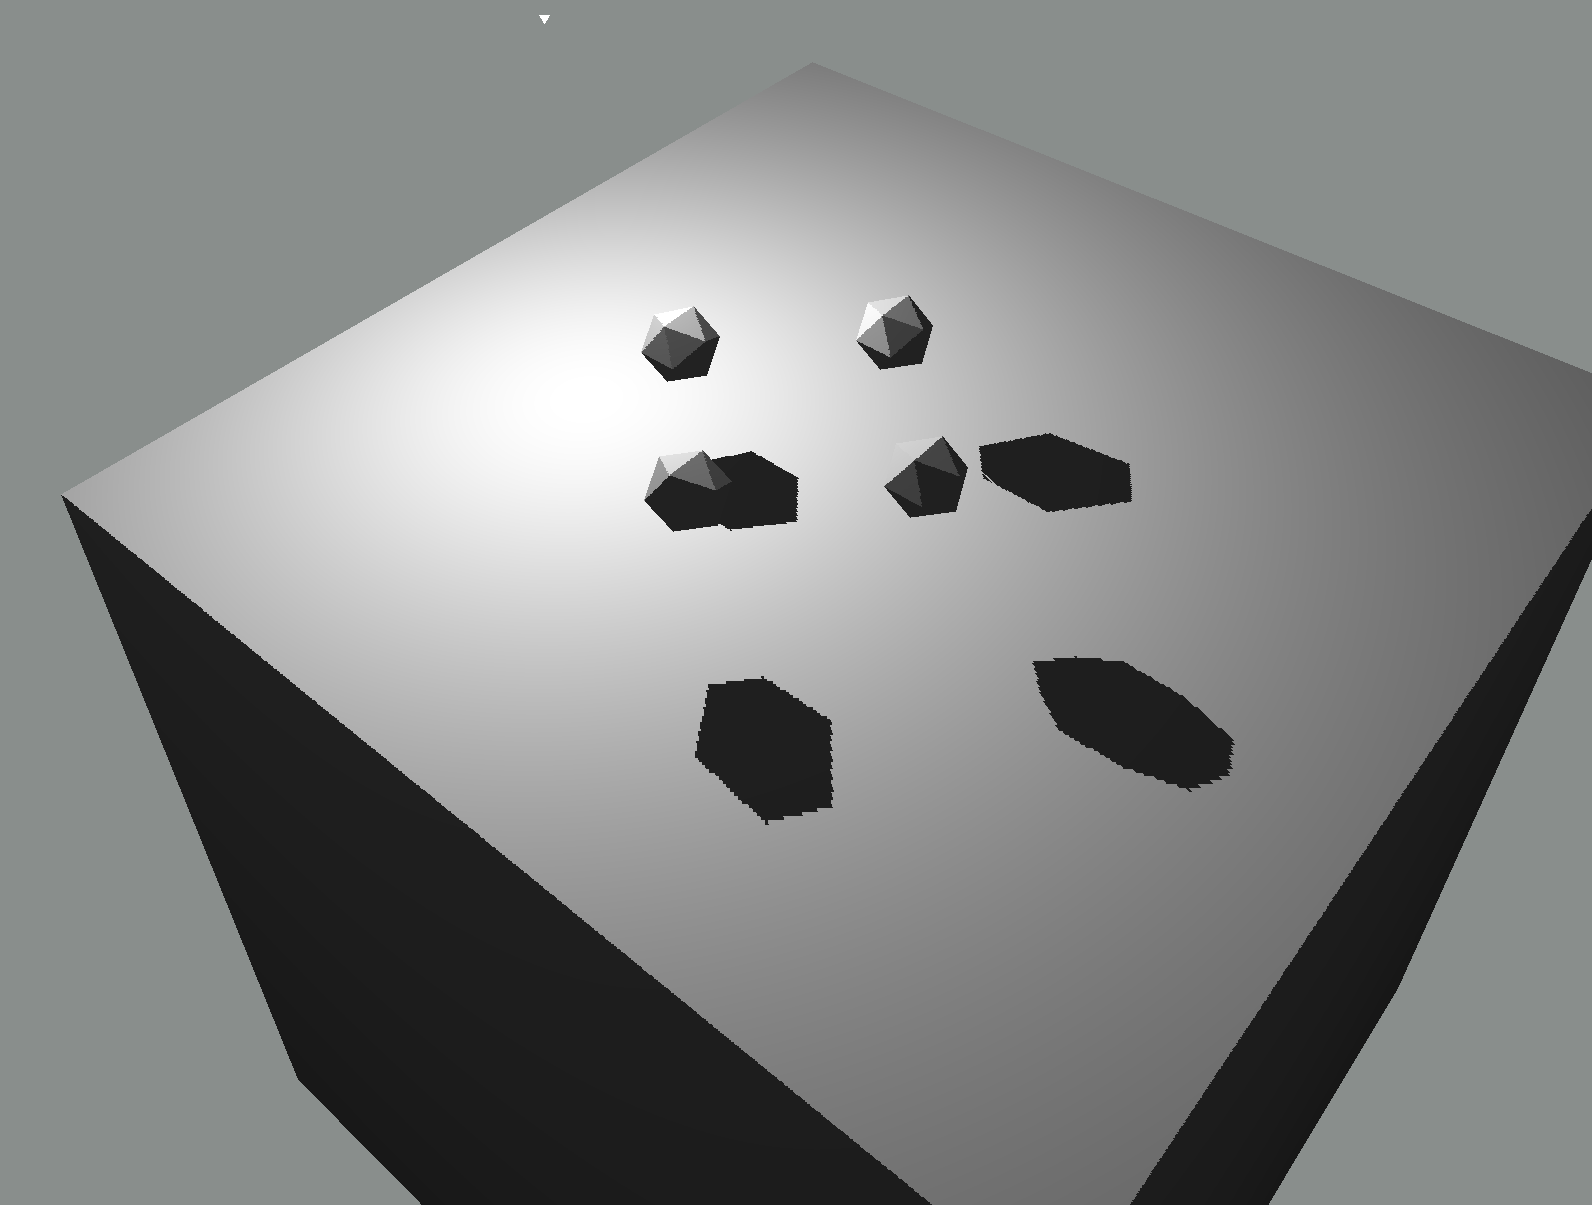
\includegraphics[width=0.3\textwidth]{light2}}
	\hfil
	\subfigure[X=3.5, Y=6, Z=3.5]{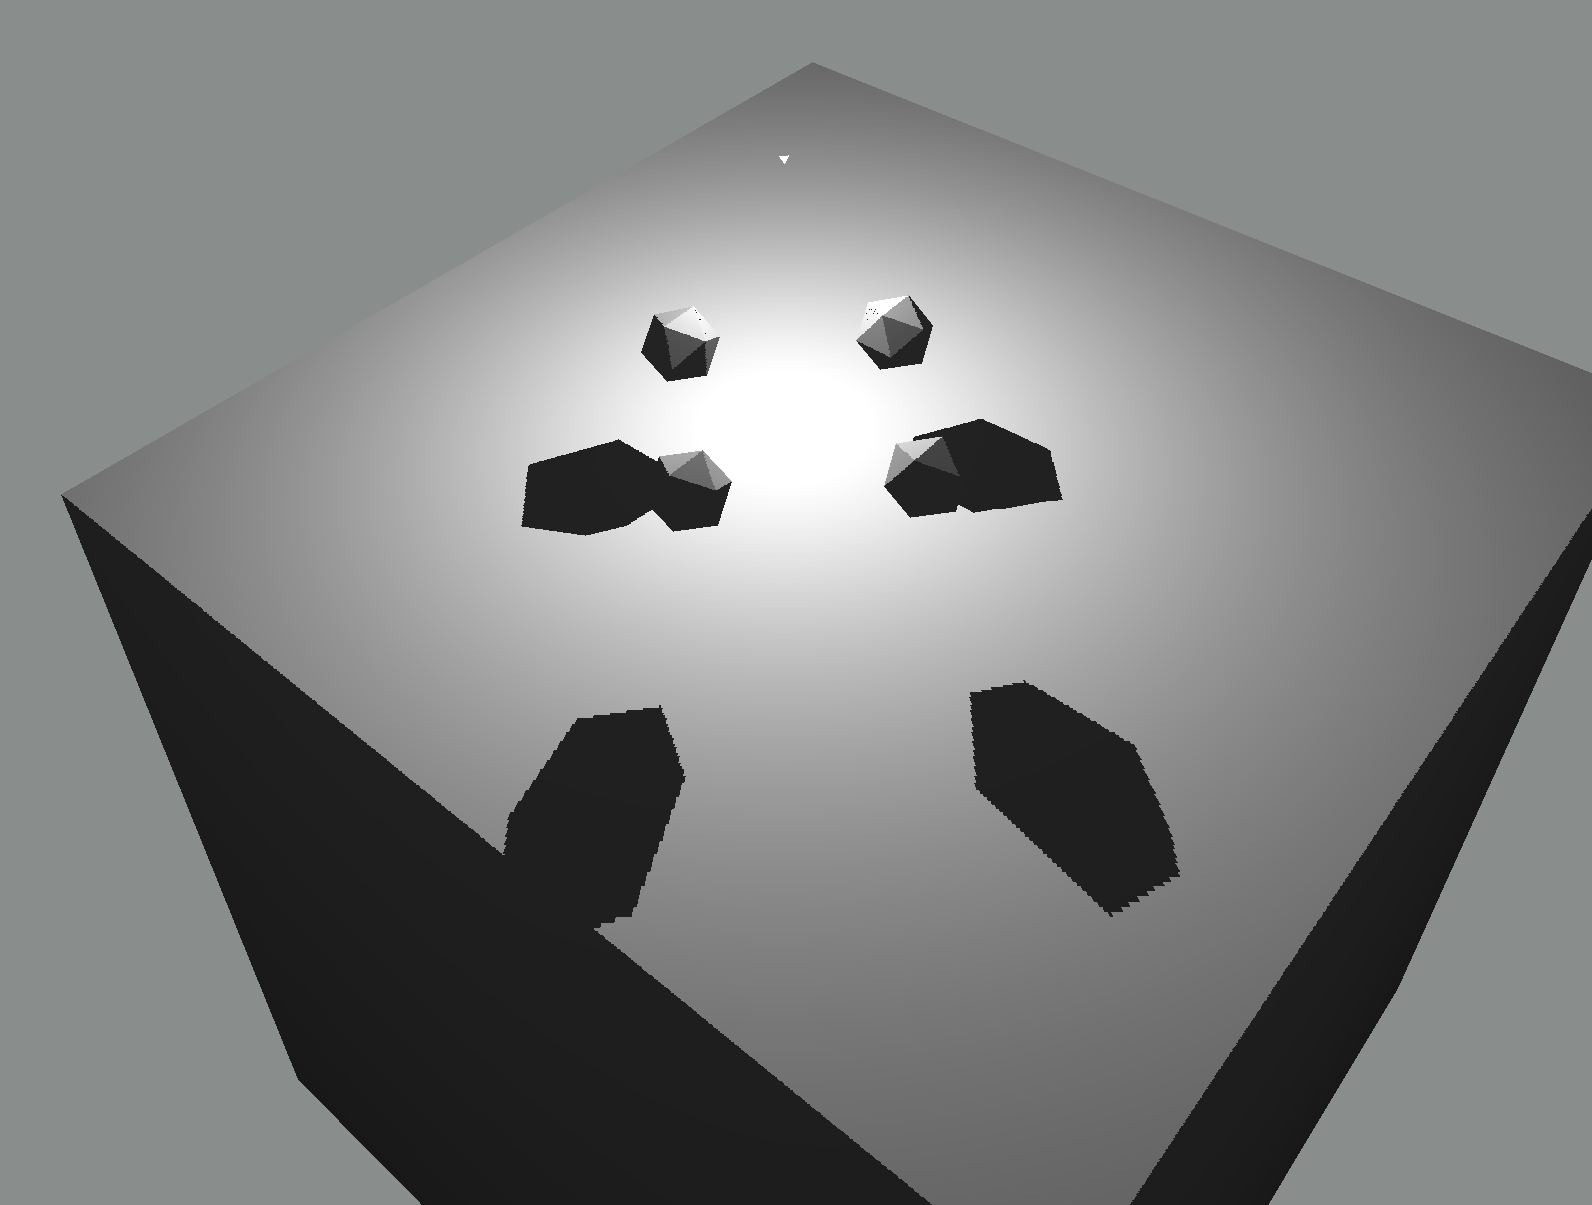
\includegraphics[width=0.3\textwidth]{light3}}
	\caption{<<Сцена при изменении положения источника света>>}
	\label{fig:light}
\end{figure}


\section*{Вывод}

В результате технологической частим было реализовано программное обеспечение с графическим интерфейсом для визуализации задачи n тел на языке программирования Go. Разработанное ПО было протестировано. Покрытие кода модульными тестами составило 24.7\%, при этом ими были покрыты такие модули как математические модули, модули матричных преобразований, отсечения и чтения объектов.


\clearpage
